\chapter{系统设计}\label{chap:design}

本章给出 QuickBoard 的总体架构、模块划分与主要数据流，重点说明“房间入口—白板协作—公式识别”三条主链路的设计取舍。

\section{总体架构}
QuickBoard 采用前后端分离与服务拆分的架构，整体可分为三部分：前端 Web 应用、后端协作服务与 OCR 服务。前端负责 UI、画布渲染与交互；后端负责房间管理、实时消息与状态同步；OCR 服务负责图像预处理与公式识别推理。该拆分方式便于独立部署与调试，也降低了前端的计算与依赖复杂度。

\begin{figure}[htbp]
  \centering
  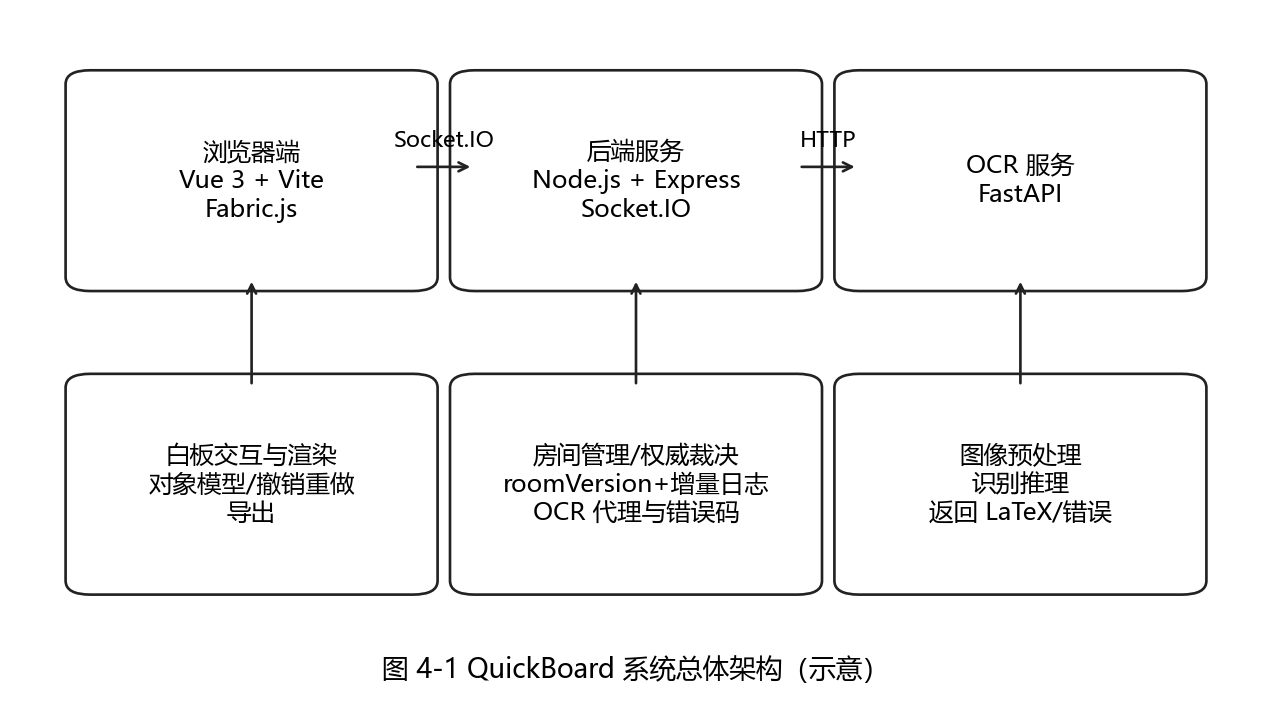
\includegraphics[width=0.92\linewidth]{figures/arch_quickboard.png}
  \caption{QuickBoard 系统总体架构}\label{fig:arch}
\end{figure}

\begin{figure}[htbp]
  \centering
  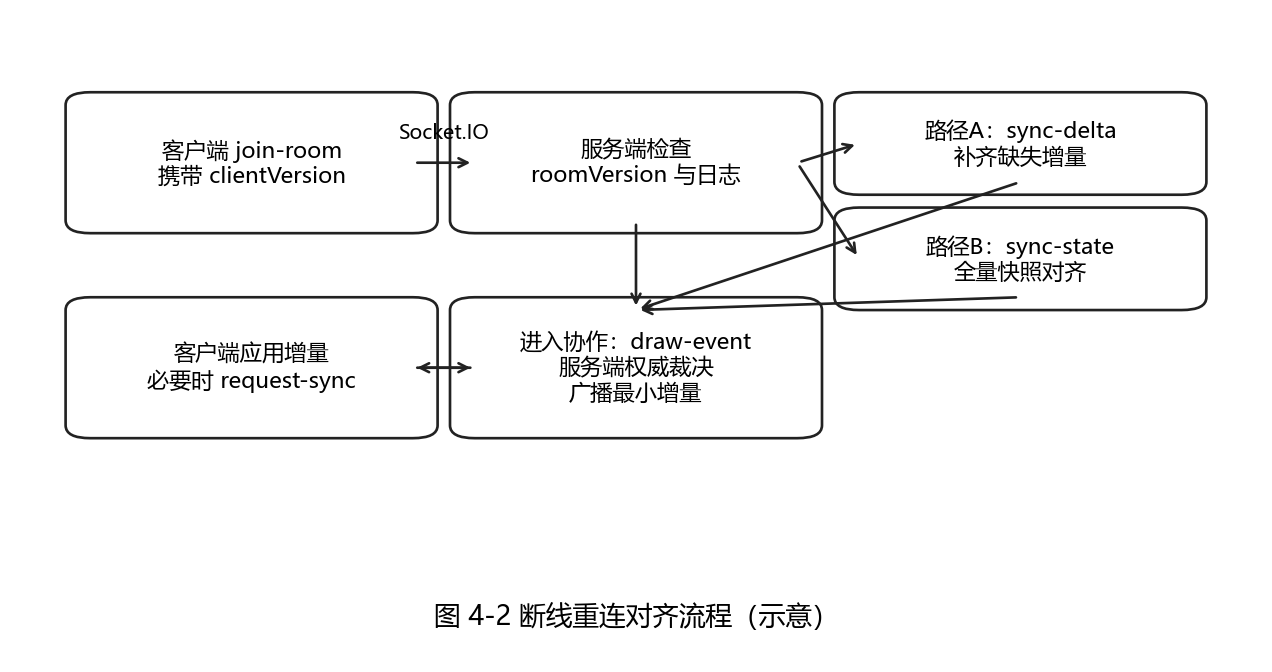
\includegraphics[width=0.92\linewidth]{figures/sync_flow.png}
  \caption{断线重连对齐流程示意}\label{fig:sync-flow}
\end{figure}

\section{模块划分}
\subsection{前端模块}
\begin{itemize}
  \item \textbf{首页模块}：提供创建房间、加入房间、最近房间管理等入口能力，并以极简布局聚焦主任务。
  \item \textbf{白板模块}：基于 Fabric.js 维护画布与对象模型，实现绘制、选择、形状、橡皮与导出等功能。
  \item \textbf{协作模块}：封装 Socket.IO 连接、房间加入、事件发送与接收，并处理断线重连与版本补包。
  \item \textbf{公式模块}：完成选区截图、识别请求、结果确认、KaTeX 渲染与双击编辑等流程。
\end{itemize}

\subsection{后端模块}
\begin{itemize}
  \item \textbf{房间管理}：维护房间生命周期与在线用户信息，支持空房间按 TTL 清理。
  \item \textbf{同步裁决}：对绘制事件进行服务端权威裁决，广播被接受的增量变更，并维护房间版本号与增量日志。
  \item \textbf{OCR 代理}：提供统一接口，将前端识别请求转发至 OCR 服务并规范化返回结构。
\end{itemize}

\subsection{OCR 服务模块}
\begin{itemize}
  \item \textbf{图像预处理}：对输入截图进行内容裁剪、尺寸对齐、反色/二值化等处理，提升识别成功率。
  \item \textbf{识别推理与回退}：优先调用公式识别模型，在失败或结果为空时对不同候选图像进行回退尝试。
  \item \textbf{结果清洗}：对输出 LaTeX 进行噪声清洗（如移除宏定义等），并对空结果统一返回错误码。
\end{itemize}

\section{关键数据流}
\subsection{创建/加入房间}
用户在首页创建房间后，前端生成房间号并进入白板页面；加入房间时，前端对输入进行归一化，支持从任意文本或链接中提取房间号并进入房间。后端根据房间号为连接分配房间上下文，并在必要时向客户端下发状态快照与增量补包。

\begin{figure}[htbp]
  \centering
  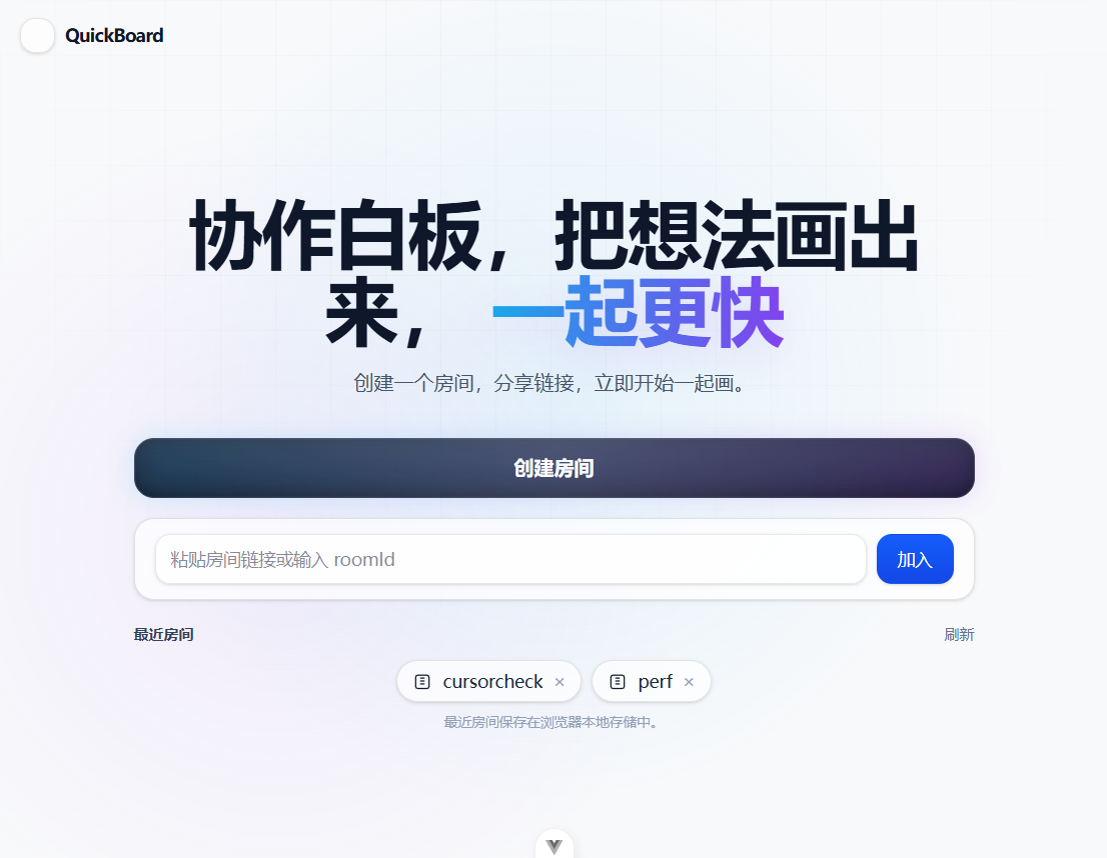
\includegraphics[width=0.9\linewidth]{figures/S1_home.png}
  \caption{系统首页入口示例}\label{fig:home}
\end{figure}

\subsection{白板协作同步}
前端对本地对象变更生成增量事件并发送至后端；后端对关键字段进行裁决后广播增量；客户端按版本号补齐缺失增量，必要时请求全量同步。该流程使协作在消息乱序与断线重连场景下仍能尽量保持一致。

\section{数据模型与事件设计}
\subsection{对象集合与字段时间戳}
系统以“对象集合”作为白板权威状态。每个对象由全局唯一 id 标识，对象属性被组织为 \texttt{data}（字段值）与 \texttt{timestamps}（字段时间戳）两部分。字段时间戳由客户端逻辑时钟生成，用于字段级 LWW 合并。删除通过写入 \texttt{\_deleted=true} 表示，并参与 LWW 比较，从而保证删除语义能够在对齐与乱序条件下自然获胜。

\subsection{核心事件}
表 \ref{tab:events} 汇总了系统主链路涉及的核心事件。事件命名与字段设计以“可解释、可对齐”为目标：对齐相关事件显式携带版本区间或权威快照，使断线窗口内的状态恢复路径明确。

\begin{table}[htbp]
  \centering
  \caption{系统核心事件汇总}\label{tab:events}
  \renewcommand{\arraystretch}{1.35}
  \begin{tabular}{lll}
    \toprule
    \textbf{事件} & \textbf{方向} & \textbf{语义与关键字段} \\
    \midrule
    join-room & C$\rightarrow$S & 加入房间，携带 userName、clientVersion \\
    draw-event & C$\rightarrow$S & 对象最小增量：id、data、timestamps \\
    sync-delta & S$\rightarrow$C & 版本补包：fromVersion、toVersion、deltas \\
    sync-state & S$\rightarrow$C & 权威快照：存活对象 + tombstones \\
    request-sync & C$\rightarrow$S & 主动请求对齐（触发快照下发） \\
    drawing-process & C$\leftrightarrow$S & 过程预览点批量（不进入权威状态） \\
    \bottomrule
  \end{tabular}
\end{table}

\subsection{公式识别与插入}
用户在白板上框选区域后，前端生成截图并调用后端识别接口；后端将请求转发至 OCR 服务并返回 LaTeX；前端展示识别结果并允许用户确认与编辑，确认后将公式作为可编辑对象插入画布并同步给其他协作者。

\subsection{错误码与 traceId 设计}
OCR 识别链路包含网络请求与模型推理，失败场景不可避免。为避免“失败无响应”或“无法解释原因”的体验断点，系统在设计上引入统一错误码与 traceId：错误码用于将失败类型显式分类（例如超时、输入无效、空结果、识别失败等），traceId 用于为一次识别请求提供跨组件关联的唯一标识。通过错误码与 traceId，前端能够给出一致且可恢复的提示，后端与 OCR 服务也能够对失败请求进行定位与排障，从而使公式能力具备工程可维护性。
